\documentclass[12pt]{article}
%\documentstyle[12pt]{article}
\setlength{\oddsidemargin}{0in}
\setlength{\evensidemargin}{0in}
\setlength{\textwidth}{6.5in}
\setlength{\topmargin}{-.3in}
\setlength{\textheight}{9in}
\pagestyle{empty}

\usepackage[super]{nth}
\usepackage{amsmath}
\usepackage{csquotes}
\usepackage{physics}
\usepackage{graphicx}% Include figure files
\usepackage{dcolumn}% Align table columns on decimal point
\usepackage{bm}
\usepackage{subfig}

\newcolumntype{L}{>{$}l<{$}}

\begin{document}

\begin{center}
{\Large Doppler-Free Saturated Absorption Spectroscopy} \\
{\Large Lab Report} \\[.3in]
{\large Bj\"{o}rn Sumner and Benjamin Crane} \\
{13 Feb 2018}
\end{center}

\section*{Motivation and Context}

The atomic hyperfine structure arises from the interaction of the nuclear and electron magnetic moments.  This structure is responsible for many technological achievements, including the development of atomic clocks.  In fact, the SI second is defined by counting the number of transitions between two hyperfine states in the cesium 133 atom \cite{NISTsec}.  Additionally, the famous 21-cm line in astronomy is generated by a hyperfine transition in interstellar hydrogen\cite{21cmPred}.

The measurement of hyperfine splittings can be performed by using Doppler-Free Saturated Absorption Spectroscopy.  We will use this technique to measure the splittings of several hyperfine structures of Rubidium.

\section*{Physics and Predictions}

\subsection*{Atomic Spectra}
Rubidium is a hydrogen-like atom with a single $5s^1$ electron in its outer shell.  This electron gives rise to the two term states we will be interested in: $5^2\text{S}_{1/2}$ and $5^2\text{P}_{3/2}$.  There are two naturally occurring isotopes of Rubidium: $72\%$ abundant ${}^{85}\text{Rb}$ with spin number $I=5/2$ and $28\%$ abundant ${}^{87}\text{Rb}$ with $I = 3/2$.
The Hamiltonian describing the atom is given by
\begin{align}
	H &= \frac{p^2}{2m} - \frac{Z_{eff} e^2}{4 \pi \epsilon_0 r} + \zeta(r) \vec{L}\cdot \vec{S} \nonumber\\
	&\qquad + \alpha \vec{J}\cdot \vec{I} + \frac{\beta}{2I(2I-1)J(2J-1)}\left[3(\vec{I}\cdot \vec{J})^2 + \frac{3}{2}(\vec{I}\cdot \vec{J}) - I(I+1)J(J+1)\right] \label{eq:hamiltonian}
\end{align}


$\frac{p^2}{2m}$ contains the kinetic energy term and $- \frac{Z_{eff} e^2}{4 \pi \epsilon_0 r}$ the standard Coulomb attractive potential.  $\zeta(r) \vec{L}\cdot \vec{S}$ is the spin orbit coupling term, which gives rise to the broad term states such as $5^2\text{S}_{1/2}$ and $5^2\text{P}_{3/2}$.  The transition between these states is $780\,\text{nm}$.  The final two terms result from the hyperfine interaction.  The former term is the hyperfine interaction between the magnetic dipole of the nucleus and electron, while the latter comes from the nuclear electric quadrupole.  These two terms will produce the hyperfine states we will explore in this lab, and we label these states by their quantum number $F$, the magnitude of the total angular momentum $\vec{F} = \vec{J} + \vec{I}$.  The possible quantum numbers vary from $\rvert J-I\rvert$ to $J+I$.  These energy levels are shown in figure \ref{fig:RbEnergy}.  In this lab, we will look at ${}^{85}\text{Rb}$ transitions from $5^2\text{S}_{1/2}\,\text{F}=3$ to $5^2\text{P}_{3/2}\, \text{F'}=1,2,3,4$ and ${}^{87}\text{Rb}$ transitions from $5^2\text{S}_{1/2}\,\text{F}=2$ to $5^2\text{P}_{3/2}\, \text{F'}=0,1,2,3$.

\begin{figure}%
	\centering
	\subfloat[${}^{85}\text{Rb}$\cite{steck85Rb}]{{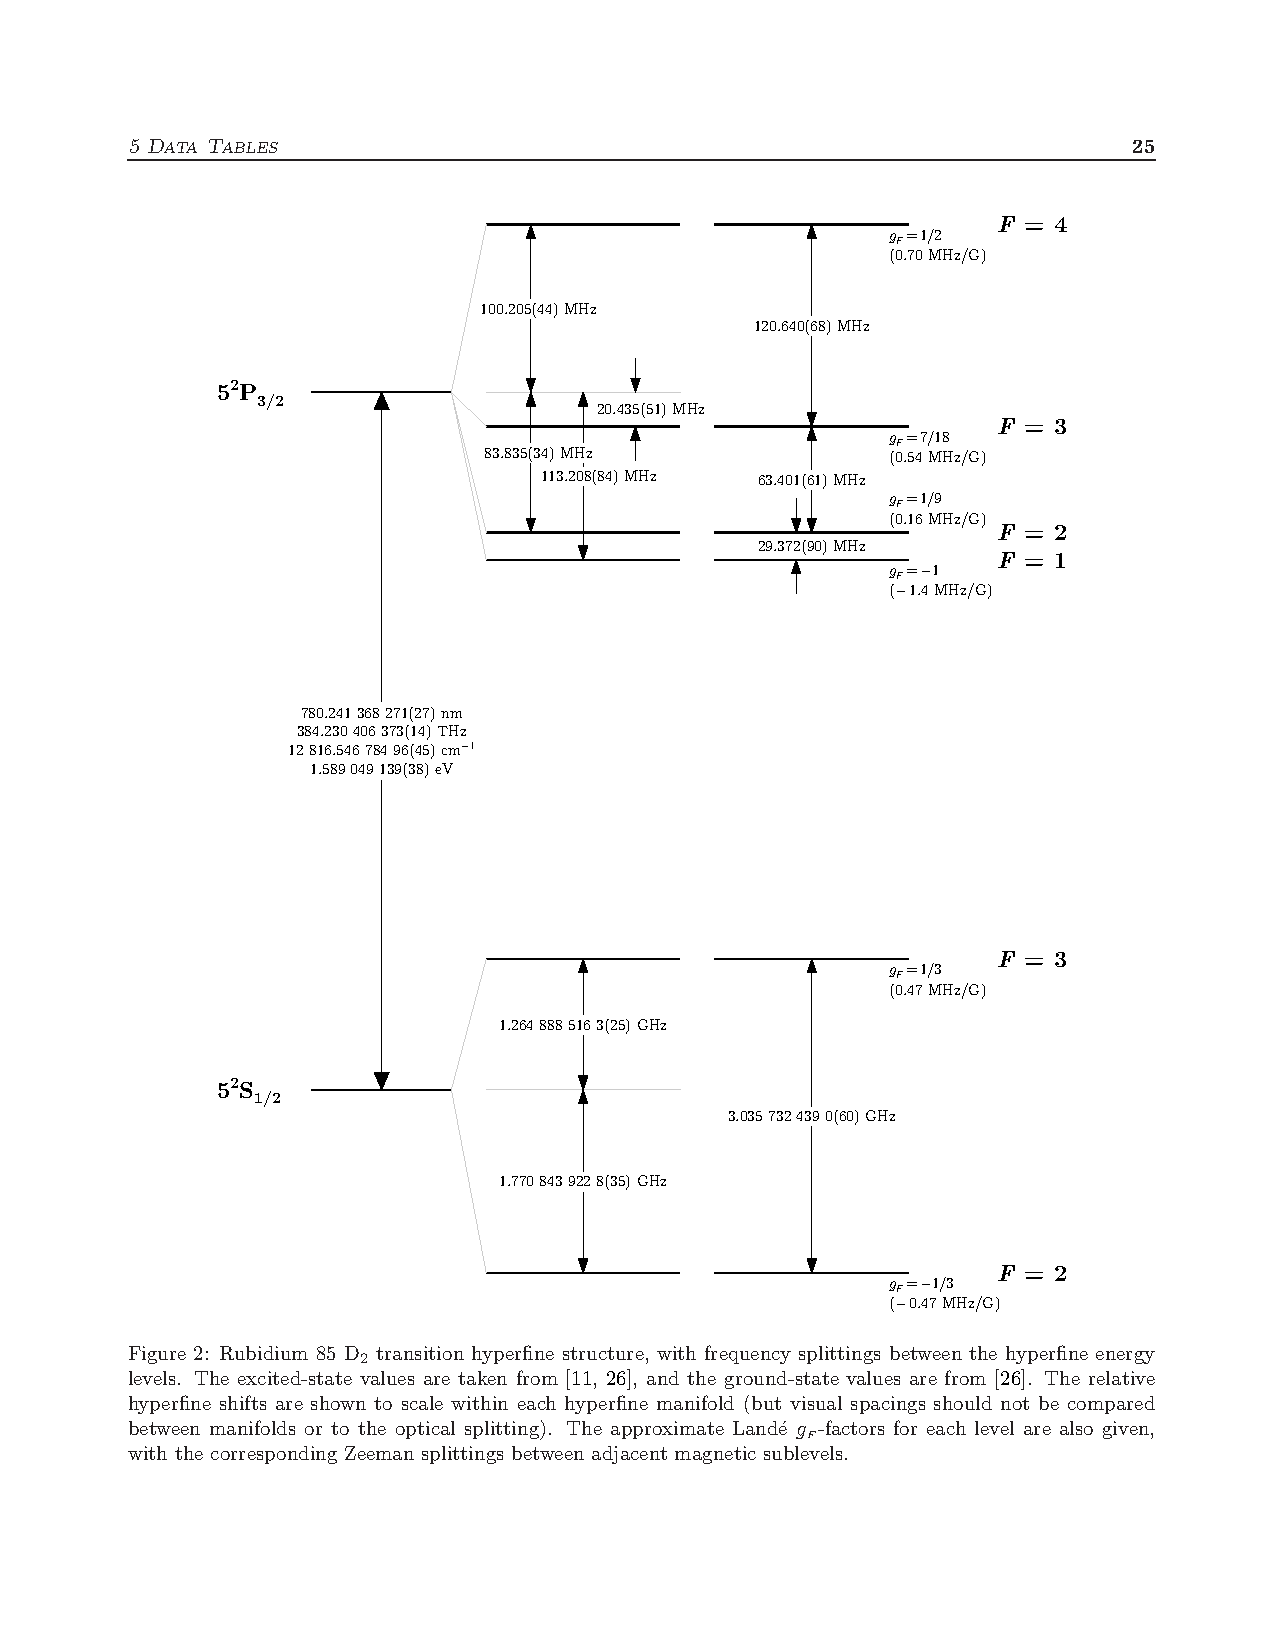
\includegraphics[width=8cm]{85D2.pdf} }}%
	\,
	\subfloat[${}^{87}\text{Rb}$\cite{steck87Rb}]{{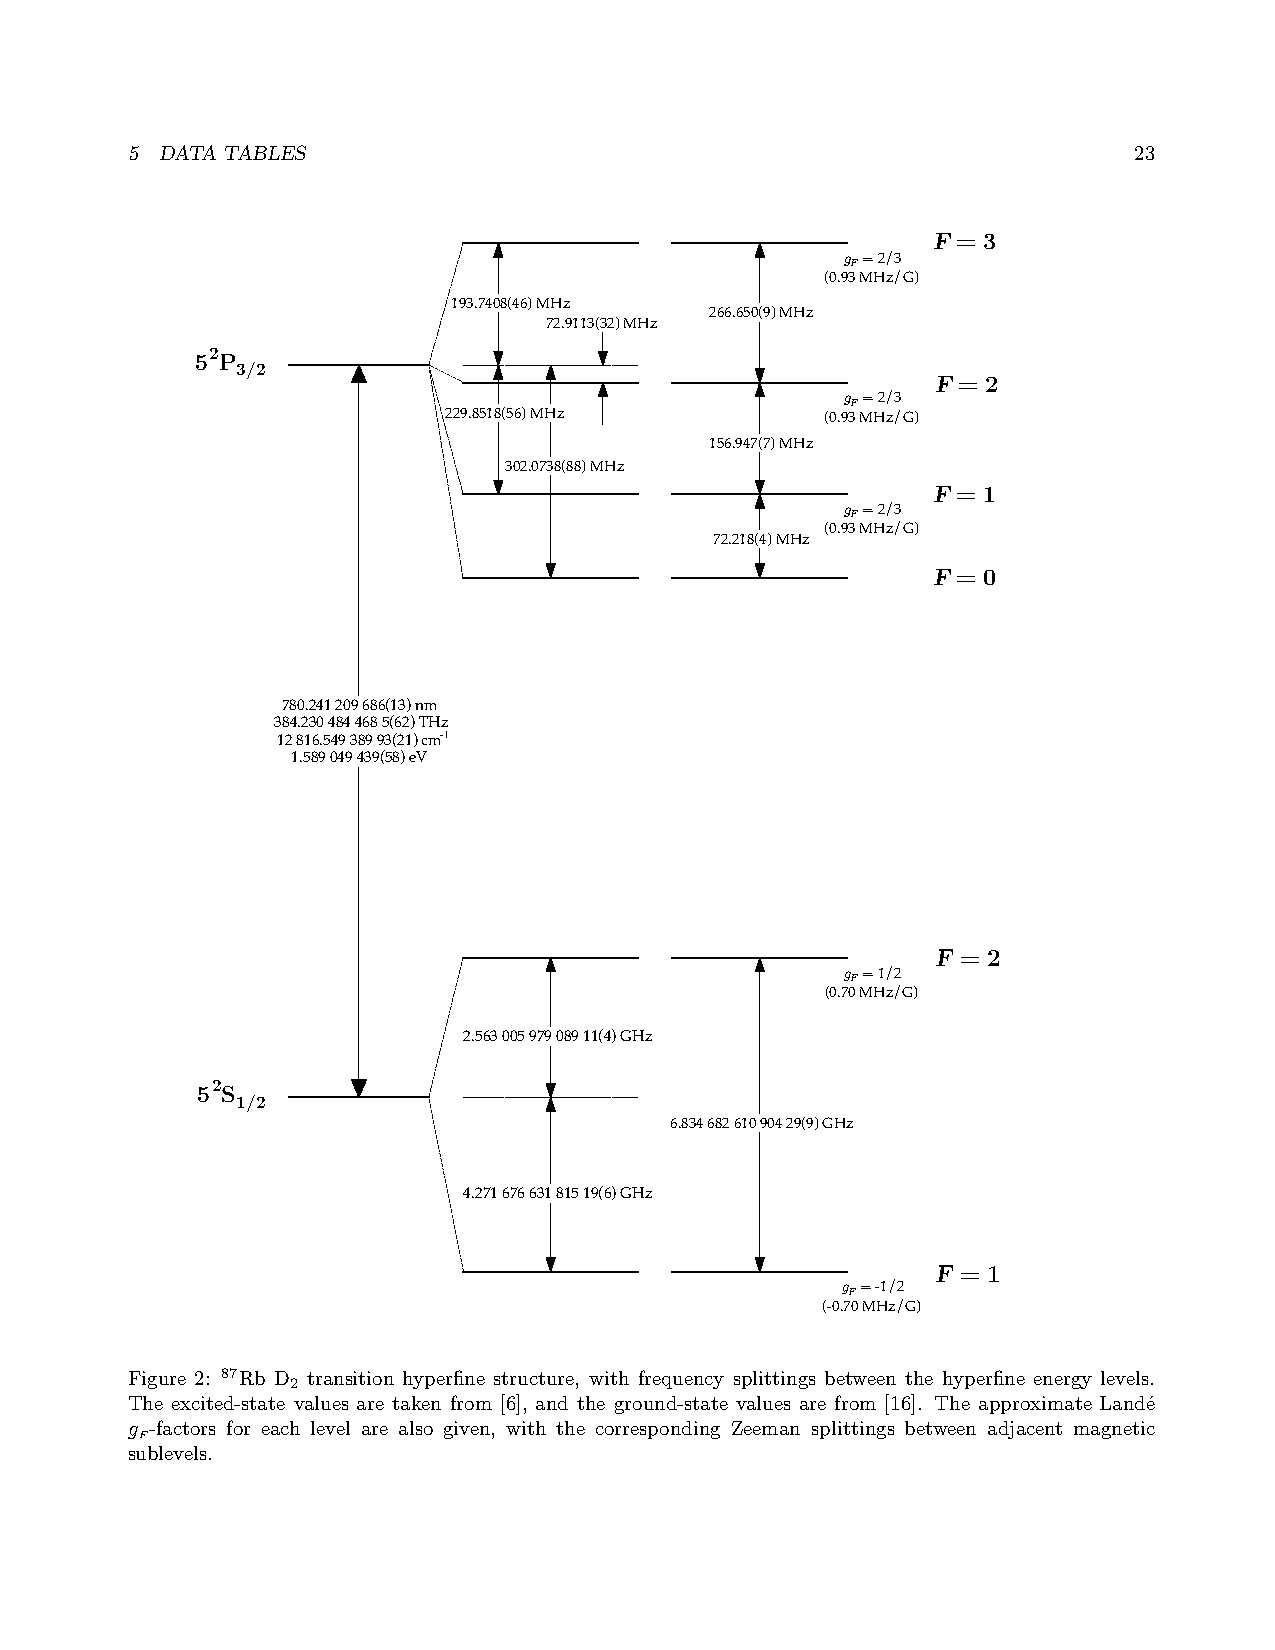
\includegraphics[width=8cm]{87D2.pdf} }}%
	\caption{Rubidium Energy Levels}%
	\label{fig:RbEnergy}%
\end{figure}

By using the Hamiltonian of equation \ref{eq:hamiltonian} in we can obtain the energies of the various hyperfine levels, and by dividing by Planck's constant, we can obtain an expression for the frequency associated with each level, indexed by quantum numbers $J$ and $F$:
\begin{align*}
	\nu_{J,F} &= \nu_J + A\frac{C}{2} + B \frac{\frac{3}{4}C(C+1) - I(I+1)J(J+1)}{2I(2I-1)J(2J-1)}
\end{align*}

where
$$C = F(F+1) - J(J+1) - I(I+1)$$

By using these formulas, we can obtain expressions in the unknown coefficients $A$ and $B$ for the `absolute' frequencies, and average these levels to get the crossover `absolute' frequencies.  Once we have these six levels, we can take the differences to obtain expressions for the splittings.  We can then use the results from our experiment to obtain values for $A$ and $B$ and compare them to the accepted values.

\subsubsection*{${}^{85}\text{Rb}\,5^2\text{P}_{3/2}\,\text{Frequencies}$}

\paragraph{$F' = 4, J = \frac{3}{2}, I = \frac{5}{2}$}
\begin{align*}
C &= \frac{15}{2}\qquad
&\nu_{\frac{3}{2},4} = \nu_J + A \frac{15}{4} + B\frac{1}{4}= \nu_J +  \frac{150A+10B}{40}
\end{align*}

\paragraph{$F' = 3, J = \frac{3}{2}, I = \frac{5}{2}$}
\begin{align*}
	C &= -\frac{1}{2}\qquad
	&\nu_{\frac{3}{2},3} = \nu_J - A \frac{1}{4} - B\frac{11}{20}= \nu_J - \frac{10A+22B}{40}
\end{align*}

\paragraph{$F' = 2, J = \frac{3}{2}, I = \frac{5}{2}$}
\begin{align*}
	C &= -\frac{13}{2}\qquad
	&\nu_{\frac{3}{2},2} = \nu_J - A \frac{13}{4} - B\frac{1}{10} = \nu_J - \frac{130A+4B}{40}
\end{align*}

\paragraph{Crossovers}
\begin{align*}
	\nu_{\bar{43}} &= \nu_J + \frac{\nu_{\frac{3}{2},4} + \nu_{\frac{3}{2},3}}{2} = \nu_J + \frac{70A-6B}{40}
\end{align*}

\begin{align*}
\nu_{\bar{42}} &= \nu_J + \frac{\nu_{\frac{3}{2},4} + \nu_{\frac{3}{2},2}}{2} = \nu_J + \frac{10A+3B}{40}
\end{align*}

\begin{align*}
\nu_{\bar{32}} &= \nu_J + \frac{\nu_{\frac{3}{2},3} + \nu_{\frac{3}{2},2}}{2} = \nu_J - \frac{70A+13B}{40}
\end{align*}

We thus obtain the following splittings:
\paragraph{Splittings}
\begin{align}
	\nu_{4}-\nu_{\bar{43}} &= 2A+\frac{2}{5}B\qquad & \nu_{\bar{43}}-\nu_{\bar{42}}= \frac{3}{2}A-\frac{9}{40}B\nonumber\\
	\nu_{\bar{42}}-\nu_{3} &= \frac{1}{2}A+\frac{5}{8}B\qquad & \nu_{3}-\nu_{\bar{32}}= \frac{3}{2}A-\frac{9}{40}B\label{eq:85splittings}\\
	\nu_{\bar{32}}-\nu_2 &= \frac{3}{2}A-\frac{9}{40}B\nonumber
\end{align}


\subsubsection*{${}^{87}\text{Rb}\,5^2\text{P}_{3/2}\,\text{Frequencies}$}

\paragraph{$F' = 3, J = \frac{3}{2}, I = \frac{3}{2}$}
\begin{align*}
C &= \frac{9}{2}\qquad
&\nu_{\frac{3}{2},3} = \nu_J + A \frac{9}{4} + B\frac{1}{4}= \nu_J +  \frac{90A+10B}{40}
\end{align*}

\paragraph{$F' = 2, J = \frac{3}{2}, I = \frac{3}{2}$}
\begin{align*}
C &= -\frac{3}{2}\qquad
&\nu_{\frac{3}{2},2} = \nu_J - A \frac{3}{4} - B\frac{3}{4}= \nu_J - \frac{30A+30B}{40}
\end{align*}

\paragraph{$F' = 1, J = \frac{3}{2}, I = \frac{3}{2}$}
\begin{align*}
C &= -\frac{11}{2}\qquad
&\nu_{\frac{3}{2},1} = \nu_J - A \frac{11}{4} + B\frac{1}{4} = \nu_J - \frac{110A-10B}{40}
\end{align*}

\paragraph{Crossovers}
\begin{align*}
\nu_{\bar{32}} &= \nu_J + \frac{\nu_{\frac{3}{2},3} + \nu_{\frac{3}{2},2}}{2} = \nu_J + \frac{30A-10B}{40}
\end{align*}

\begin{align*}
\nu_{\bar{31}} &= \nu_J + \frac{\nu_{\frac{3}{2},3} + \nu_{\frac{3}{2},1}}{2} = \nu_J - \frac{10A-10B}{40}
\end{align*}

\begin{align*}
\nu_{\bar{21}} &= \nu_J + \frac{\nu_{\frac{3}{2},2} + \nu_{\frac{3}{2},1}}{2} = \nu_J - \frac{70A+10B}{40}
\end{align*}

We thus obtain the following splittings:
\paragraph{Splittings}
\begin{align}
\nu_{3}-\nu_{\bar{32}} &= \frac{3}{2}A+\frac{1}{2}B\qquad & \nu_{\bar{32}}-\nu_{\bar{31}}= A-\frac{1}{2}B\nonumber\\
\nu_{\bar{31}}-\nu_{2} &= \frac{1}{2}A+B\qquad & \nu_{2}-\nu_{\bar{21}}= A-\frac{1}{2}B \label{eq:87splittings}\\
\nu_{\bar{21}}-\nu_1 &= A-\frac{1}{2}B\nonumber
\end{align}

\subsection*{Doppler Broadening}

The spectra given in the previous section are obtained from a description of nature in the atom's frame of reference with no external effects.  However, real Rubidium atoms are subject to thermal motion, and as such these spectral lines will undergo broadening owing to the motion of the atoms relative to the laser.  Atoms moving toward the laser will `see' radiation blue shifted, and so absorption will only occur if the incoming photons are of a lower frequency than predicted by the spectra in figure \ref{fig:RbEnergy}.  Similarly, atoms moving away from the laser will absorb photons of higher frequency.  Because the velocity of these atoms follows the Maxwell distribution, it can be expected that the spectral lines will similarly follow such a distribution.  It can be shown that the half width of these distributions is given by 
\begin{align}
	\Delta \nu_{1/2} &= 2\frac{\nu_0}{c}\sqrt{\frac{2kT}{M}\ln(2)}
\end{align}

where $\nu_0$ is the rest frame atomic resonance, $M$ is the mass of the atom and $T$ is the temperature of the sample.

We can use this to predict the expected half width of the D2 lines.  Using figures from Steck\cite{steck85Rb}\cite{steck87Rb},

\subsubsection*{${}^{85}\text{Rb}\,\text{D}_2$}

\begin{align}
	\Delta \nu_{1/2} &= \frac{2}{\lambda_0}\sqrt{\frac{2kT}{M_{85}}\ln(2)}\nonumber\\
	&= \frac{2}{780.241\,\text{nm}}\sqrt{\frac{2\left(1.381\times10^{-23}\,\frac{\text{J}}{\text{K}}\right)\left(293\,\text{K}\right)}{1.410\times10^{-25}\,\text{kg}}\ln(2)}\nonumber\\
	&\approx 511 \text{MHz} \label{pred:85D2}
\end{align}

\subsubsection*{${}^{87}\text{Rb}\,\text{D}_2$}

\begin{align}
\Delta \nu_{1/2} &= \frac{2}{\lambda_0}\sqrt{\frac{2kT}{M_{87}}\ln(2)}\nonumber\\
&= \frac{2}{780.241\,\text{nm}}\sqrt{\frac{2\left(1.381\times10^{-23}\,\frac{\text{J}}{\text{K}}\right)\left(293\,\text{K}\right)}{1.443\times10^{-25}\,\text{kg}}\ln(2)}\nonumber\\
&\approx 505 \text{MHz}\label{pred:87D2}
\end{align}

These broadened spectra mask the hyperfine structure of the atoms, and so we must use Doppler-Free Saturated Absorption Spectroscopy to tease out these individual spectra.

\subsection*{Doppler-Free Saturated Absorption Spectroscopy}

To isolate the hyperfine structure, we use saturation absorption spectroscopy.  When a probe beam passes through the rubidium sample, thermal motion of the atoms will result in absorption of this beam across a range of frequencies, as these frequencies will be blue-shifted or red-shifted to the atomic resonance owing to the motion of the atoms relative to the probe source.  However, if we were to use a strong pump beam to saturate the absorption across the entire frequency range, then both beams will be on resonance at the transition frequency for a subpopulation of the atoms that have velocities perpendicular to the propagation direction of the lasers.  These atoms can then undergo \textit{stimulated} emission from the probe beam, and thus the absorption will be reduced (the photodetector will register a stronger signal) at the transition frequency.  By using an additional probe beam separate from the overlap, we can subtract the signals to obtain the Doppler-free saturated absorption signal.

As an added bonus, this strong pump beam also favors the higher ground state in both isotopes ($F=3$ for ${}^{85}\text{Rb}$, $F = 2$ for ${}^{87}\text{Rb}$), which promotes the D$_2$ line we are interested in observing.

An additional feature of this form of spectroscopy are the presence of `crossover peaks'.  These peaks arise from the pump beam depopulating the ground state on atoms on resonance with the pump's red- or blue-shifted light.  However, at the crossover frequencies, these atoms are on a different resonance with the probe beam's blue- or red-shifted light.  This means that the probe beam will not be absorbed by these atoms, since they are already excited by the pump beam.  Since this effect happens for atoms with opposite velocities, this effect occurs for a larger part of the atomic population, and so we expect these crossover peaks to be stronger than those of the actual hyperfine levels.

\subsection*{Michelson Interferometer}

Though we can obtain a plot of voltage against time, we must have a way of comparing the time differences in the signals to an associated frequency.  We can use a Michelson interferometer to calibrate our signal.  By precisely measuring the different leg lengths of the interferometer, then a time-varying frequency of light entering the interferometer will produce a time-varying intensity of its recombined beams.  It can be shown that the frequency spacing of the interference maxima is given by

\begin{align}
	\Delta \nu &= \frac{c}{2 \Delta L}\label{eq:interferometer}
\end{align}

Thus, by using the period of the interferometer signal which is associated with a frequency span, we have a way of measuring the frequency spacings of interest from the spectroscopy signals.

\section*{Experiment and Data}

\subsection*{Experimental Setup}
We designed the experimental setup on the optical table to accommodate both Doppler-Free Saturated Absorption Spectroscopy and the Michelson Interferometer for calibration.  Using the infrared camera and the hand held card viewer allowed us to trace the paths of laser beam. The laser was directed through a cube beam splitter with one path continuing towards the Michelson Interferometer setup, and the other towards a thick beam splitter. The thickness of the beam splitter allows for spatially separated but parallel beams directly through the Rubidium vapor sample. These two weak beams are called the reference probe beam and the overlapping probe beam. The main portion of the laser continued straight through the thick beam splitter, becoming the start of the pump beam. The strong pump beam was angled with a mirror towards the opposite end of the table and was then angled with a separate mirror to overlap a probe beam. These two beams are propagating in opposite directions. The overlapping probe beam continues through the rubidium vapor sample and is then directed with a mirror onto the photodetector. The reference probe beam is also reflected from a mirror through an optical attenuator and onto a separate photodetector. To achieve comparable power from the two probe beams we used a translation stage holding the variable attenuator to reduce the intensity of the reference beam. This was done visually with the aid of the oscilloscope  displaying the two channels of the photodetectors. 

The beam passing through the first beam splitter is incorporated into the Michelson Interferometer.  This interferometer consists of a thin microscope slide at $\approx45^{\circ}$ to act as a 50-50 beam splitter. The longer reflected leg of the Michelson Interferometer has a measured length of 388.5 $\pm $0.5 mm, while the shorter leg is measured to have a length of 94.5 $\pm $0.5mm. The laser traveled down and back each leg of the Michelson Interferometer and recombined at the beam splitter before continuing to the photodetector.  We ensured the beams were parallel and occupying the same space by using a card to ensure there was no divergence from the recombination point to the far wall approximately 3 meters away. After orienting the mirrors, beam splitters and photodetectors we noticed an odd feedback signal superimposed on both probe signals on our oscilloscope. After discussing the feedback with Professor Jun Ye, we were able to determine the feedback was a result of the interferometer beams entering into the spectroscopy component of the table. To negate these effects we installed another variable optical attenuator at an angle between the cube splitter and microscope slide to prevent the interferometer signal from entering the spectroscopy setup.  This eliminated the anomalous addition from the probe beam signals.  Using the Math function of the oscilloscope we were able to subtract the Doppler-broadened spectral lines with hyperfine structure (overlapping probe) from the Doppler-broadened spectral lines (reference probe) we were able to display just the specific peaks of the hyperfine structure. See figure \ref{fig:Layout} for a picture of our optical table.

\begin{figure}[h!]
	\centering
	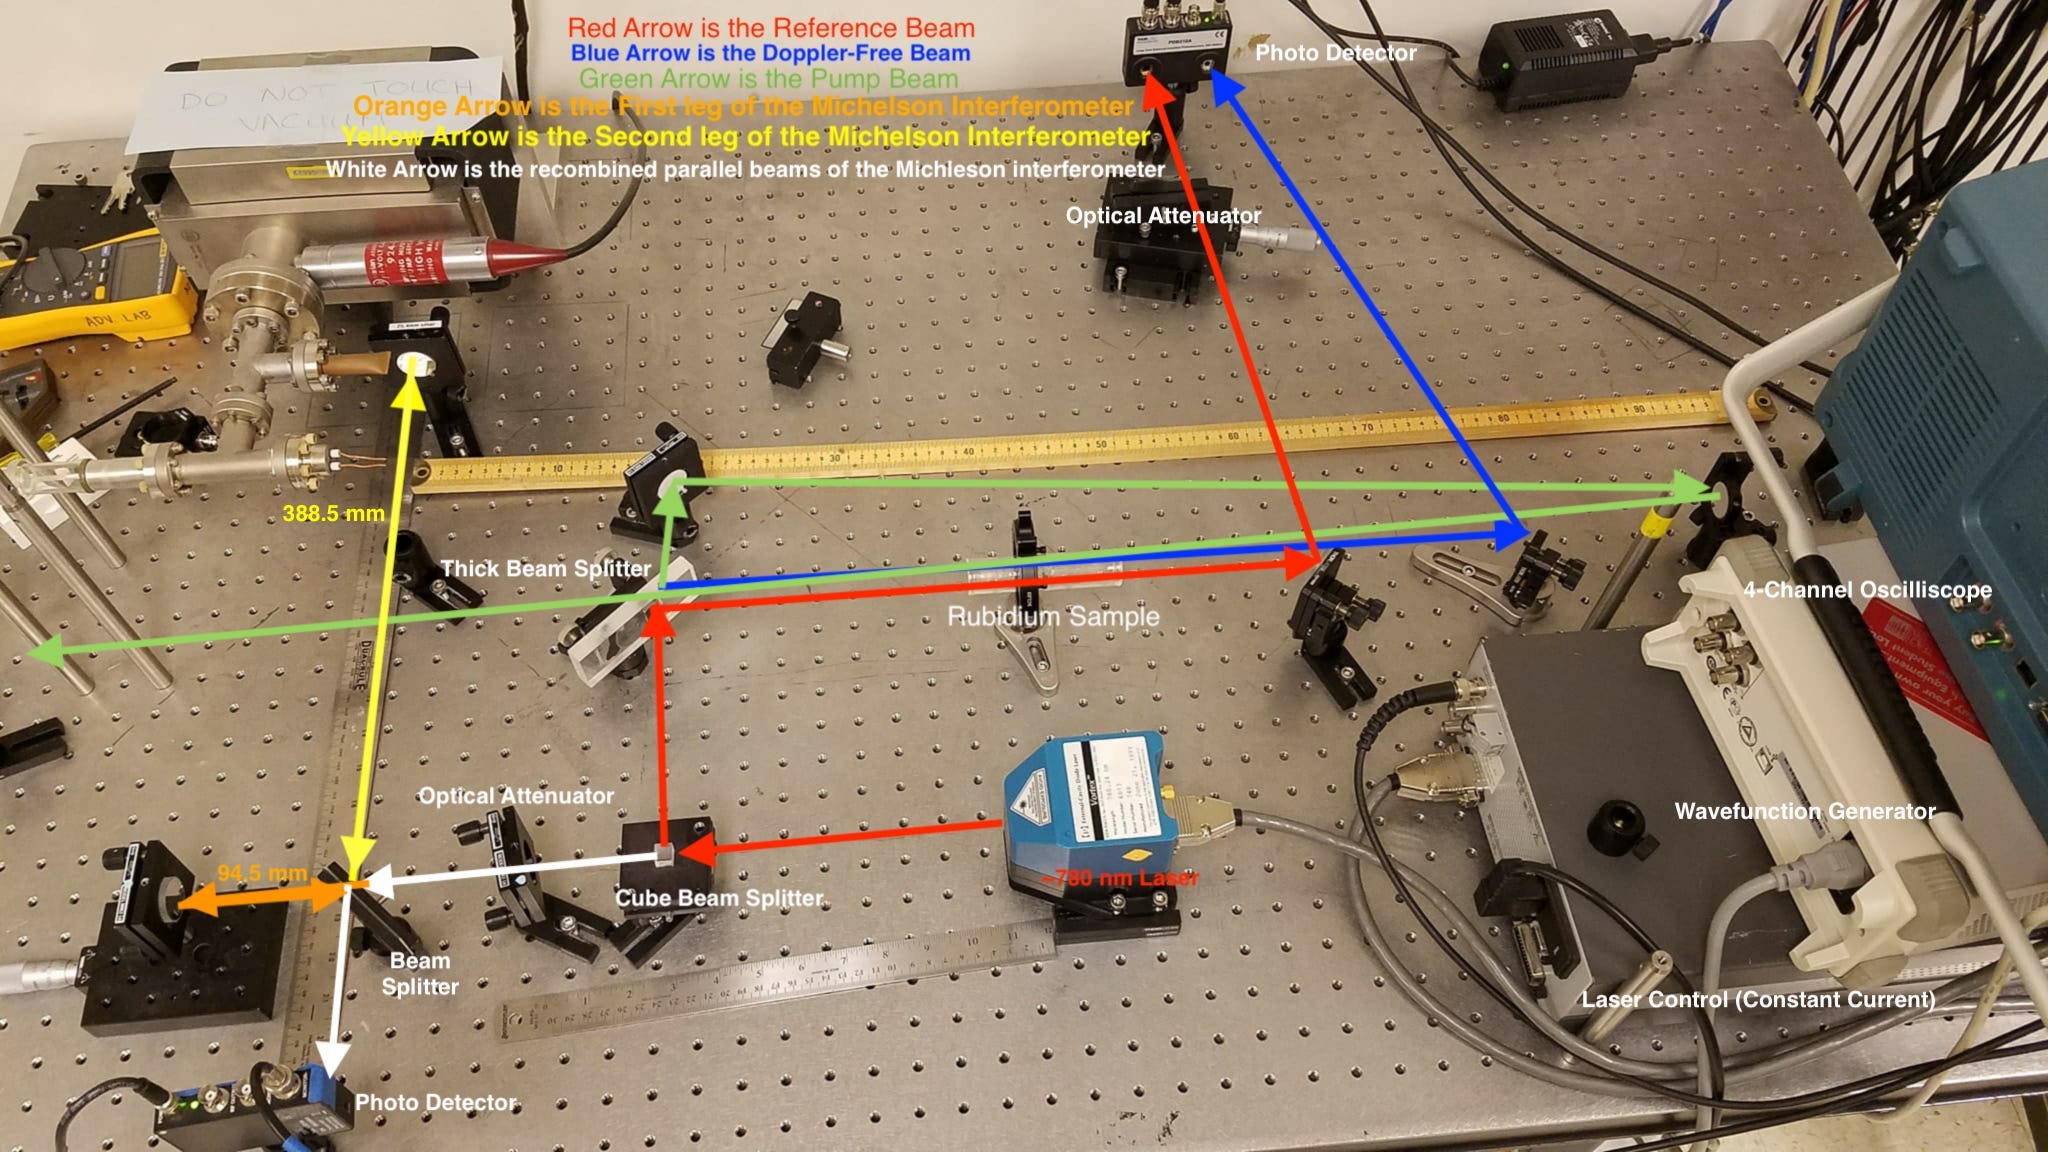
\includegraphics[width=\textwidth]{DFS_Layout.jpg}
	\caption{Experiment Layout}%
	\label{fig:Layout}%
\end{figure}

Toggling the Vortex Laser controls for the voltage and the wave-function generator's frequency and peak-to-peak ramp voltage allowed for panning left and right and zooming in and out on specific portions, focusing on the hyperfine splitting of the 5$^2P_{3/2} $ states.  We decided to arrange the output from the Michelson Interferometer to be displayed along side the three other signals, allowing for a direct comparison. These signals included the reference probe beam, the pump-overlapped probe beam, the interferometer signal and the ramp voltage signal upon which the oscilloscope is triggered.  By incorporating all of the signals onto the same oscilloscope we were able to directly compare all signals.

This allowed us to measure the full width at half maximum (FWHM) of the Doppler broadened lines of both isotopes as well as the separation of the hyperfine states for the D$_2$ lines of both isotopes. We then were able to solve for the constants A and B of the 5$^2 P_{3/2}$.

A critical feature of our setup was the careful alignment of the pump beam.  By ensuring the maximum overlap of the pump beam with one of the probe beams, we maximized the population in the higher ground states as well as the population of atoms interacting simultaneously with both pump and probe beams.  This optimizes the amount of stimulated hyperfine transitions that occur, making our signals much clearer.

\subsection*{Results and Discussion}

Two representative sets of data for the D$_2$ transitions for both ${}^{85}\text{Rb}$ and ${}^{87}\text{Rb}$ are shown in figure \ref{fig:RbOsc}.  As can be seen from figure \ref{fig:RbOsc}, we were able to isolate 4 of the 6 ${}^{85}\text{Rb}$ D$_2$ hyperfine transitions (3 transitions, 3 crossovers), but all 6 D$_2$ transitions for ${}^{87}\text{Rb}$. 

\begin{figure}%
	\centering
	\subfloat[${}^{85}\text{Rb}$]{{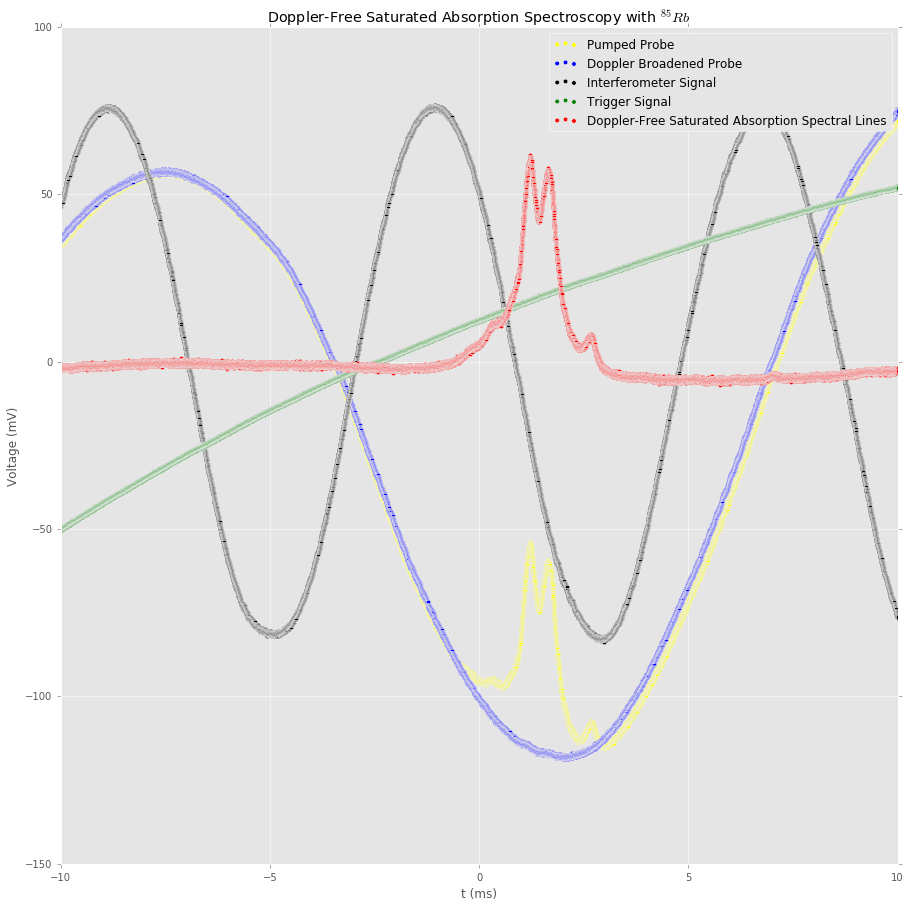
\includegraphics[width=8cm]{../Screenshots/85RbReport.png} }}%
	\,
	\subfloat[${}^{87}\text{Rb}$]{{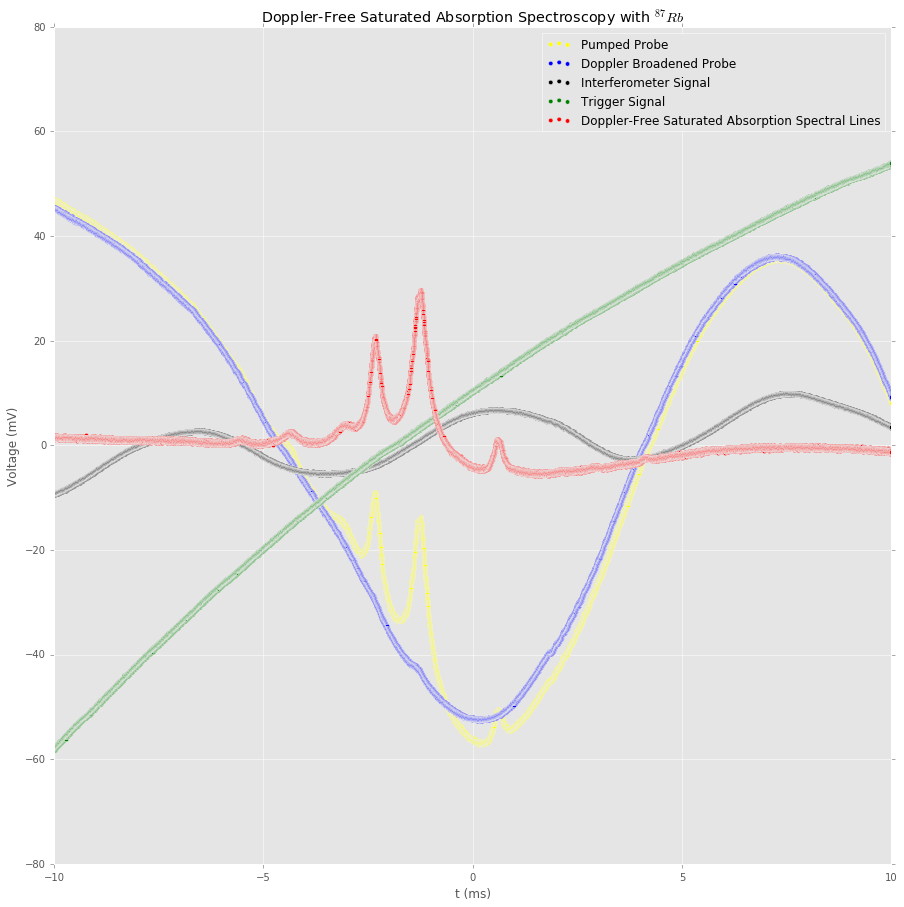
\includegraphics[width=8cm]{../Screenshots/87RbReport.png} }}%
	\caption{Rubidium D$_2$ Oscilloscope Data}%
	\label{fig:RbOsc}%
\end{figure}

We first obtain our `meterstick' for measuring frequency spacings.  To do this, we curve fit the interferometer signal to a cosine, and obtain a fitted period, $\Delta t$.  We then compare spacings relative to this `meterstick' by observing that the ratio of the frequency spacing we desire, $f$ to the interferometer frequency spacing $\Delta \nu$ must equal the ratio of the time-spacing between the signals of interest $\tau$ to the time spacing of the interferometer period $\Delta t$:
$$ \frac{f}{\Delta \nu}= \frac{\tau}{\Delta t}$$
By using equation \ref{eq:interferometer}, we obtain:
\begin{align}
	f &= \frac{c}{2\Delta L \Delta t}\tau \label{eq:meterstick}
\end{align}

By performing the curve fitting mentioned above, we find a `meterstick' time of $\Delta t_{85} = 7.7884\pm 0.0004$ ms for ${}^{85}\text{Rb}$, and $\Delta t_{87} = 7.325\pm 0.001$ ms for ${}^{87}\text{Rb}$.  Given the lengths of the interferometer, we use $\Delta L = 0.2940$ m.

\begin{figure}%
	\centering
	\subfloat[${}^{85}\text{Rb}$]{{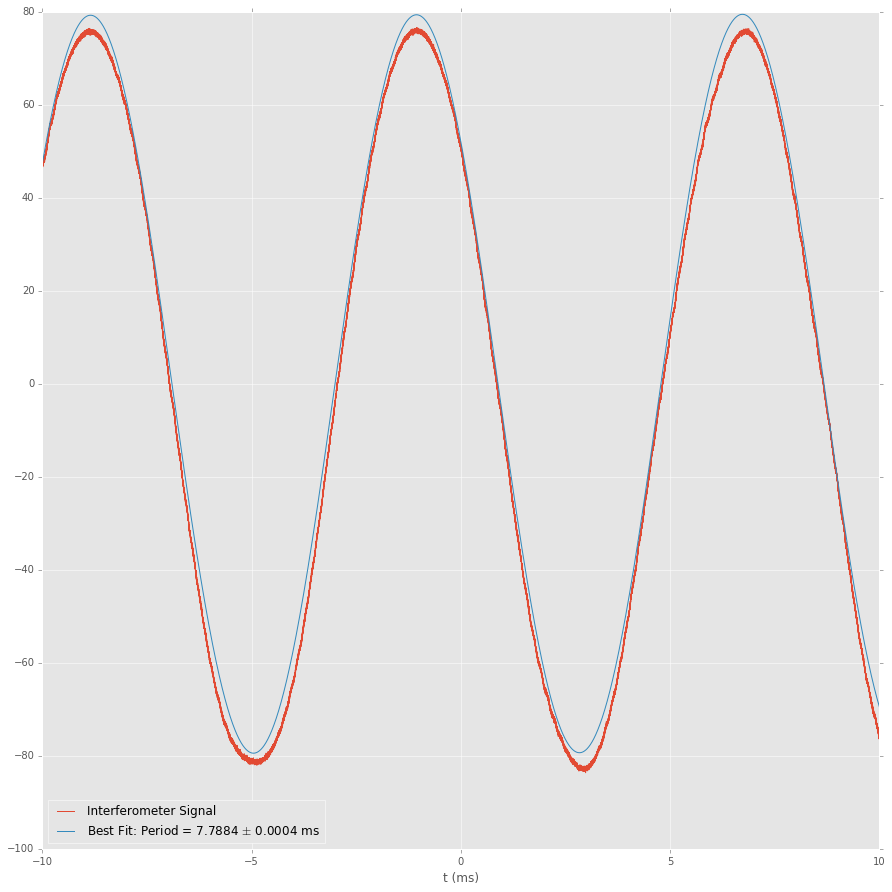
\includegraphics[width=8cm]{../Screenshots/85Rb_fringe.png} }}%
	\,
	\subfloat[${}^{87}\text{Rb}$]{{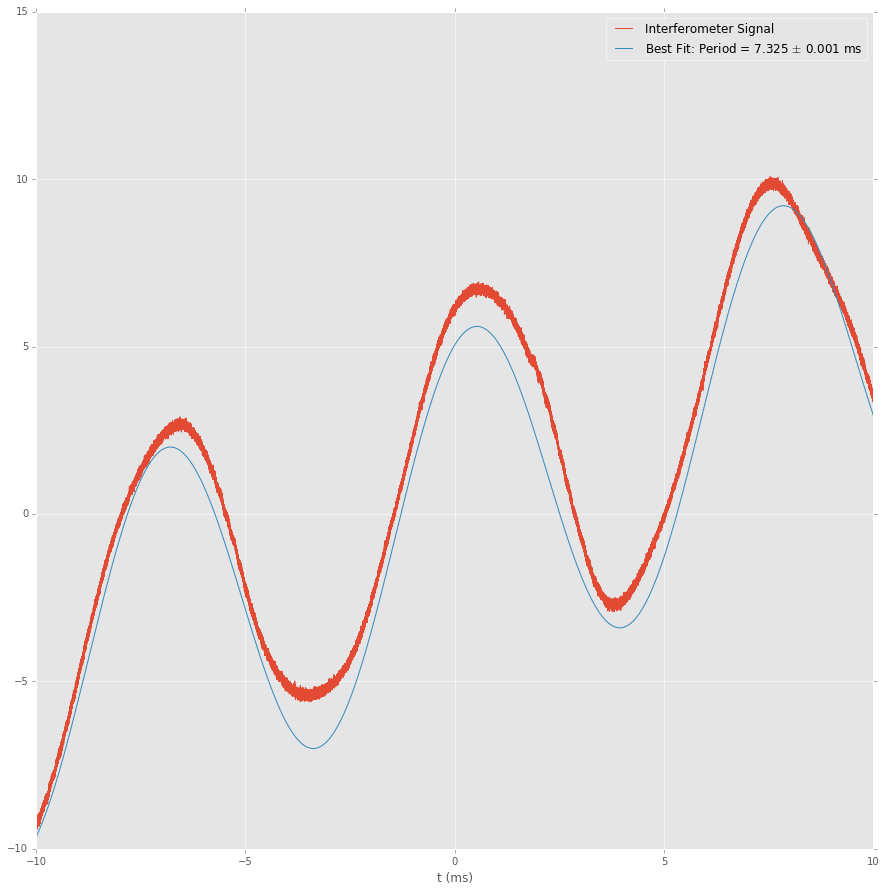
\includegraphics[width=8cm]{../Screenshots/87Rb_fringe.png} }}%
	\caption{Interferometric `Metersticks'}%
	\label{fig:meterstick}%
\end{figure}

The data and fitting functions are shown in figure \ref{fig:meterstick}.  We attribute the difference in precision to the presence of more consistent nature of the ${}^{85}\text{Rb}$ signal.  Additionally, there is a time dependent component of the DC offset of the interferometer signal.  We did not have the time to further explore the nature of this signal, but we must remain cautious of results we obtain based on this signal.  The number of fringes are limited by the length difference in the interferometer arms, per equation \ref{eq:interferometer}.  We use these numbers in equation \ref{eq:meterstick} to obtain the following results.

\subsubsection*{FWHM of Doppler broadened D$_2$ lines}

We would like to measure the FWHM of the Doppler broadened D$_2$ transition.  We do this by fitting the Doppler broadened probe signals to Gaussians, and then using the relation $FWHM = 2 \sqrt{2 \ln(2)}\sigma$, where $\sigma$ is the standard deviation of the fitted Gaussian.  The data and the fitted function are shown in figure \ref{fig:FWHM}.

\begin{figure}%
	\centering
	\subfloat[${}^{85}\text{Rb}$]{{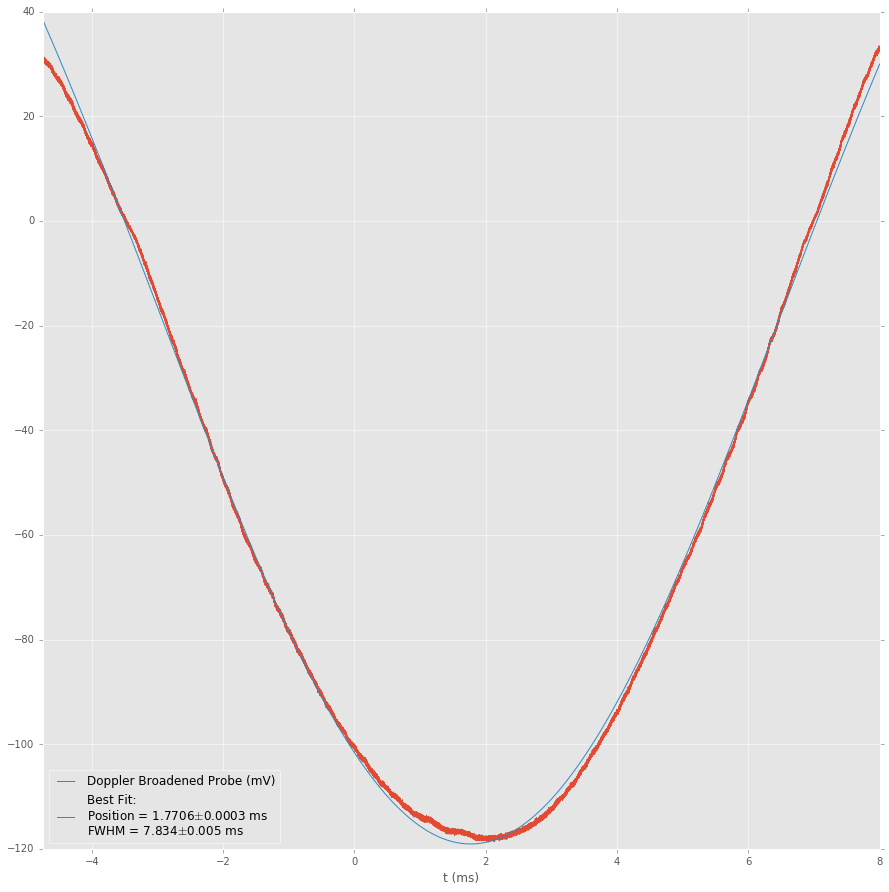
\includegraphics[width=8cm]{../Screenshots/85RbFWHM.png} }}%
	\,
	\subfloat[${}^{87}\text{Rb}$]{{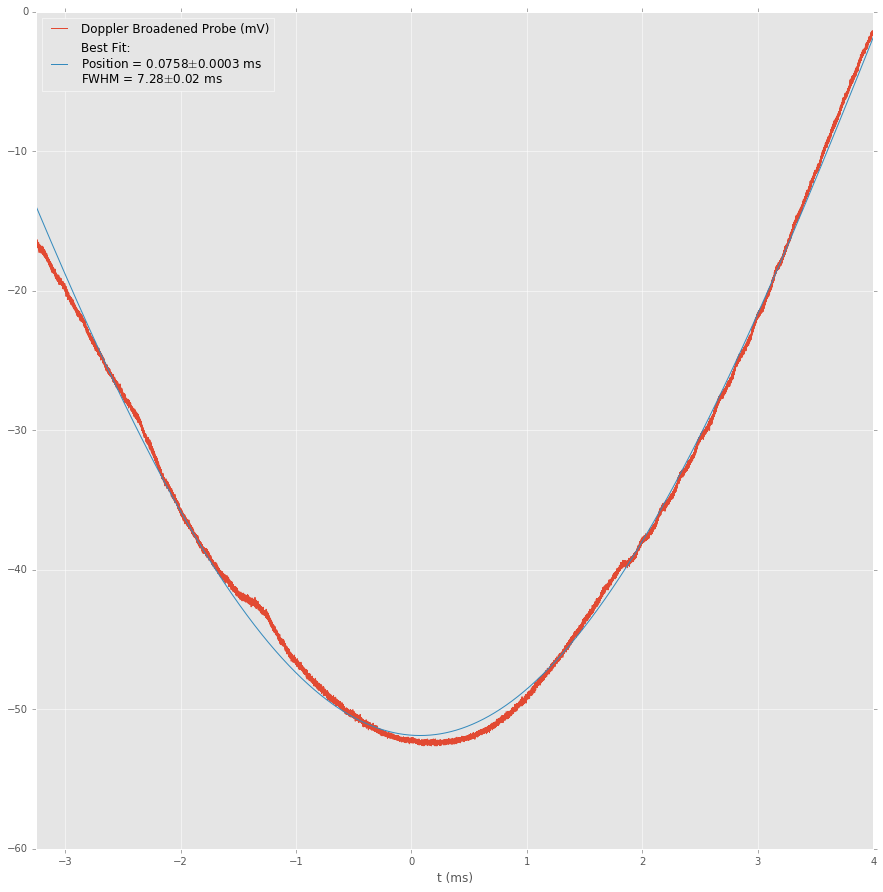
\includegraphics[width=8cm]{../Screenshots/87RbFWHM.png} }}%
	\caption{Full Width at Half Maximum fitting of Doppler Broadened D$_2$ lines}%
	\label{fig:FWHM}%
\end{figure}

These fittings produce the following results:  For ${}^{85}\text{Rb}$, we get a FWHM frequency range of $512.8\pm0.2$ MHz.  This agrees quite well with the predicted value of $511$ MHz in equation \ref{pred:85D2}.  For ${}^{87}\text{Rb}$, we find $506\pm1$ MHz, again agreeing with the predicted $505$ MHz in equation \ref{pred:87D2}.  However, we must acknowledge the sensitivity of these figures to the fitting of the Gaussian to the data.  Here, we eyeballed the data window for which to determine our fitting function.  There are additional signals in the windows that came from other transitions that we did not wish to include in the fitting, and thus we felt justified in excluding this data from the fitting.

\subsubsection*{Hyperfine Line Splittings}

We assume a Gaussian fit for the individual peaks for the individual hyperfine transitions.  We determined the locations of the peaks shown in figure \ref{fig:HyperfineOverview} by fitting the peaks, and again, attempting to judiciously choose which data to include in the fit, we obtained the center of each peak and used these data to obtain the following hyperfine splittings

\begin{figure}%
	\centering
	\subfloat[${}^{85}\text{Rb}$]{{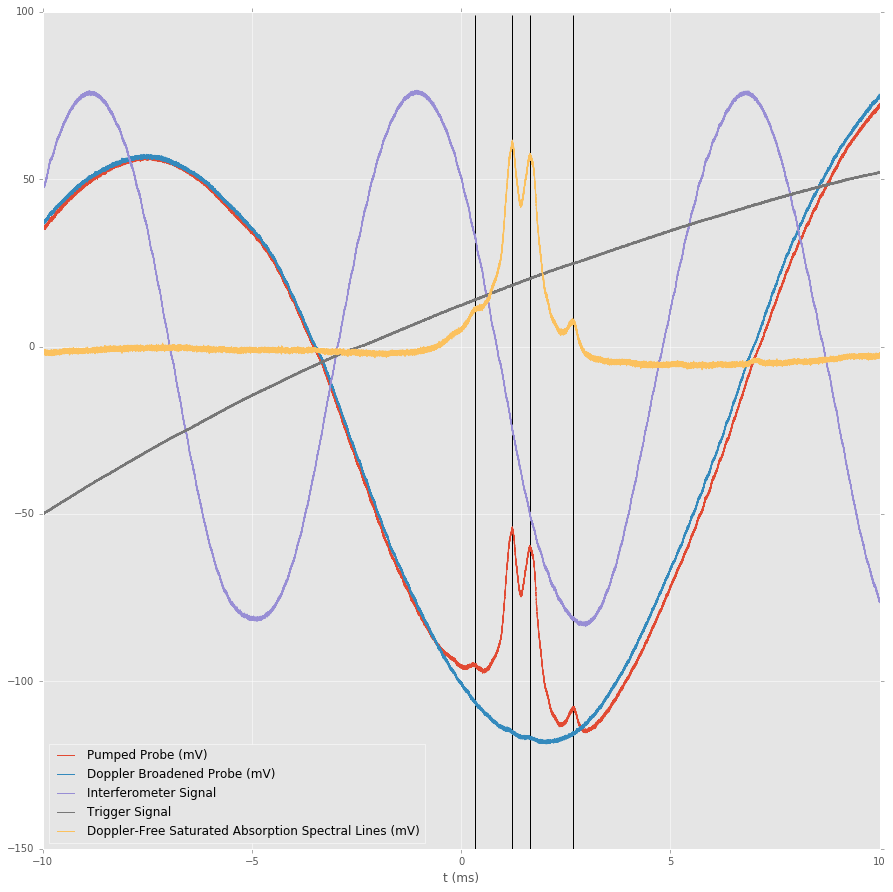
\includegraphics[width=8cm]{../Screenshots/85Rb_allpeaks.png} }}%
	\,
	\subfloat[${}^{87}\text{Rb}$]{{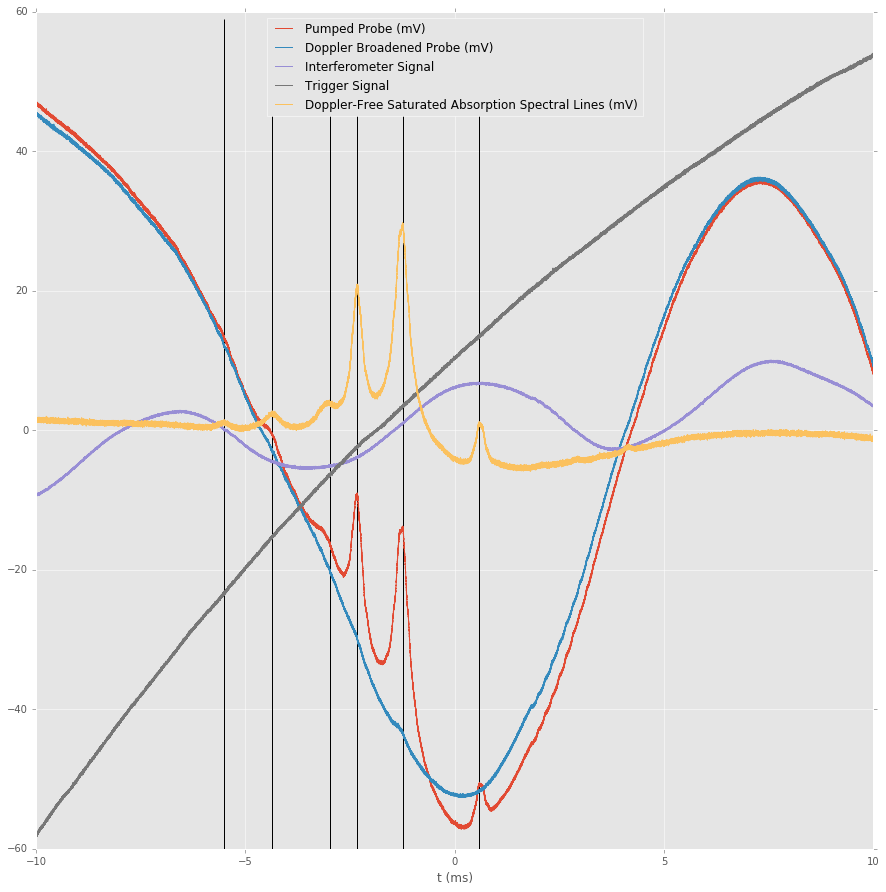
\includegraphics[width=8cm]{../Screenshots/87Rb_allpeaks.png} }}%
	\caption{Overview of locations of hyperfine peaks}%
	\label{fig:HyperfineOverview}%
\end{figure}

Individual fittings for the peaks of each D$_2$ line can be found in figures \ref{fig:85Hyperfine} and \ref{fig:87Hyperfine}.  We find the following splittings amongst the peaks discernible from the spectra, and compare them to the agreed upon values, from Steck\cite{steck85Rb}\cite{steck87Rb}:

\begin{center}
	\begin{tabular}{| L|c | L|c |L|c|}
		\hline
		{}^{85}Rb\textbf{ Splittings} & \textbf{Value (MHz)} & \textbf{Measured (MHz)}\\ 
		\hline
		\nu_{4}-\nu_{\bar{43}} & 60.3200 &  66.173\pm0.001\\ 
		\hline
		\nu_{\bar{43}}-\nu_{\bar{42}} & 31.7005 & 28.36\pm0.02\\ 
		\hline
		\nu_{\bar{42}}-\nu_{3} & 28.6195 & 51.48\pm0.07\\ 
		\hline
		\nu_{3}-\nu_{\bar{32}} & 31.7005 & \\ 
		\hline
		\nu_{\bar{32}}-\nu_2 & 31.7005 & \\
		\hline
	\end{tabular}
\end{center}
	\vspace{5mm}
\begin{center}
	\begin{tabular}{| L|c | L|c |L|c|}
		\hline
		{}^{87}Rb\textbf{ Splittings} & \textbf{Value (MHz)} & \textbf{Measured (MHz)} \\ 
		\hline
		\nu_{3}-\nu_{\bar{32}} & 133.3250 &130.82\pm0.03\\ 
		\hline
		\nu_{\bar{32}}-\nu_{\bar{31}} & 78.4735 & 73.79\pm0.03\\ 
		\hline
		\nu_{\bar{31}}-\nu_{2} & 54.8515 & 48.29\pm0.02\\ 
		\hline
		\nu_{2}-\nu_{\bar{21}} & 78.4735 & 93.42\pm0.05\\ 
		\hline
		\nu_{\bar{21}}-\nu_1 & 78.4735 & 81.68\pm0.07\\
		\hline
	\end{tabular}
\end{center}

The most notable discrepancy are the missing splittings from the ${}^{85}$Rb D$_2$ line.  However, we noticed that the expected spacings in ${}^{85}$Rb D$_2$ are less than half of those of ${}^{87}$Rb D$_2$.  We thus attribute the absence of lines to the close proximity they are in, requiring a greater resolution to discern individual peaks.  We argue that the peaks are present, but lost amongst each other owing to the amplitude and width of adjacent peaks.

Additionally, we wish to point out that the most prominent peaks in the spectra of both isotopes correspond to the crossover frequencies, as predicted by theory.


\begin{figure}[ht!]
	\begin{center}
		%
		\subfloat[Peak 1]{%
			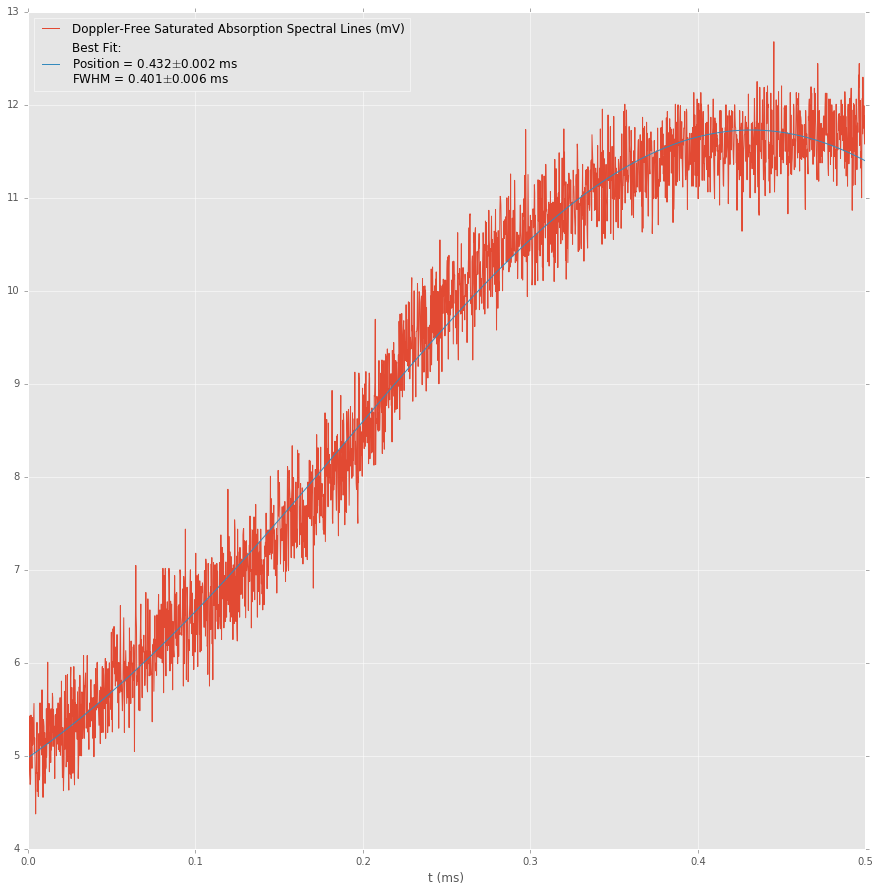
\includegraphics[width=8cm]{../Screenshots/85Rb_peak1.png}
		}%
		\subfloat[Peak 2]{%
			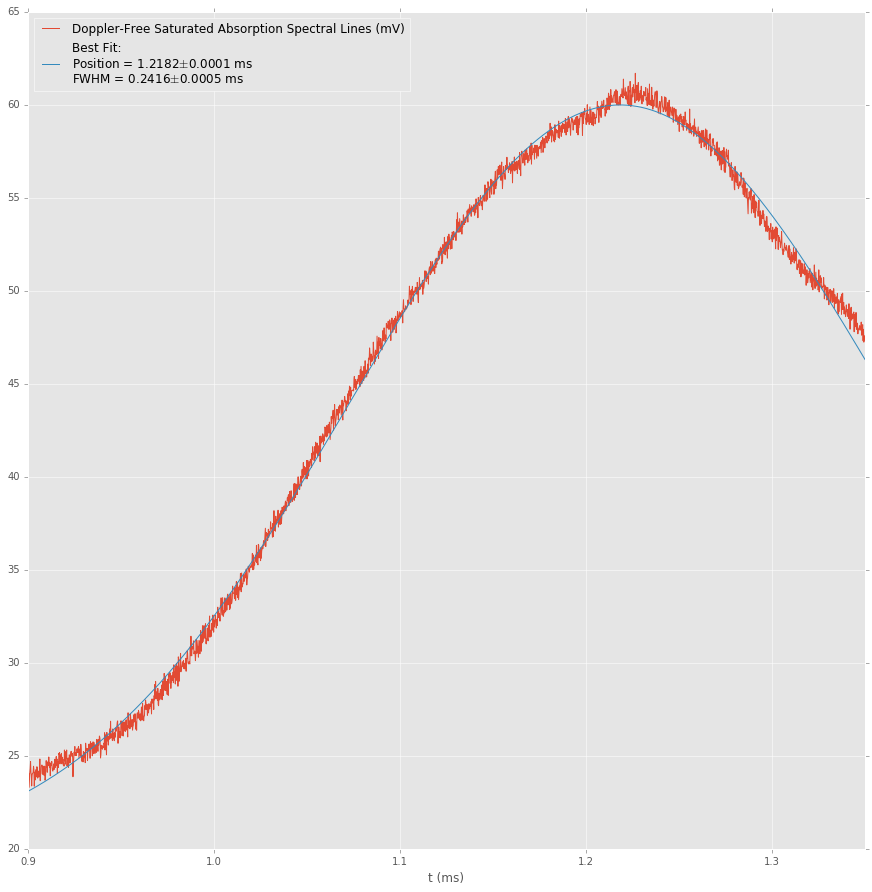
\includegraphics[width=8cm]{../Screenshots/85Rb_peak2.png}
		}\\ %  ------- End of the first row ----------------------%
		\subfloat[Peak 3]{%
			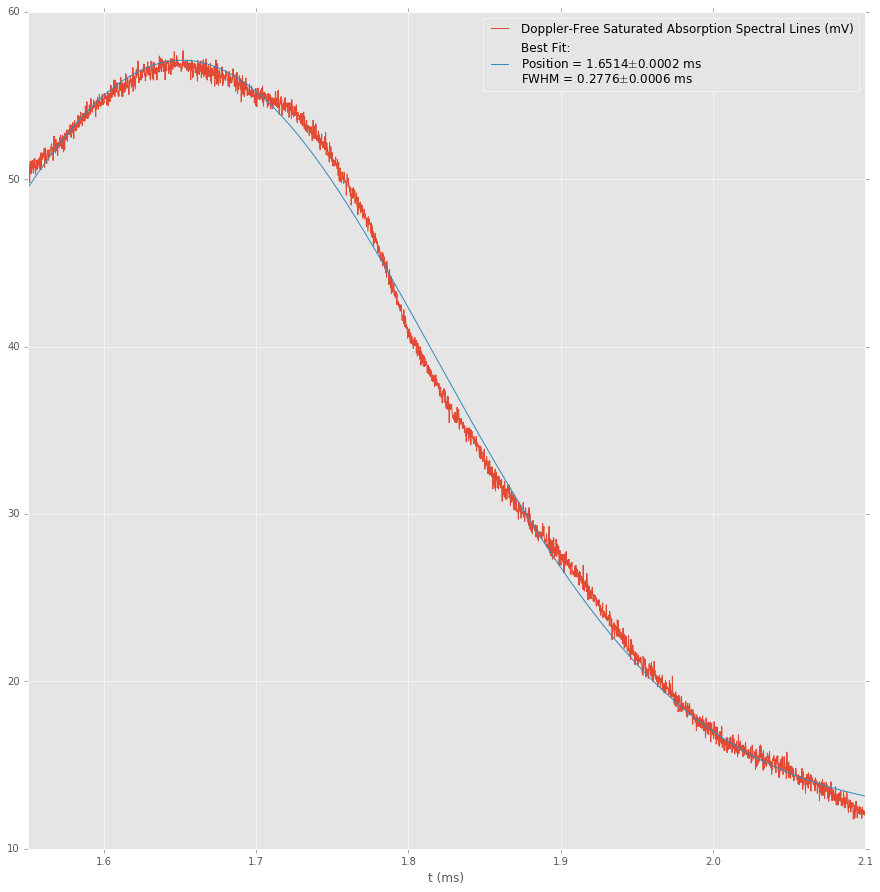
\includegraphics[width=8cm]{../Screenshots/85Rb_peak3.png}
		}%
		\subfloat[Peak 4]{%
			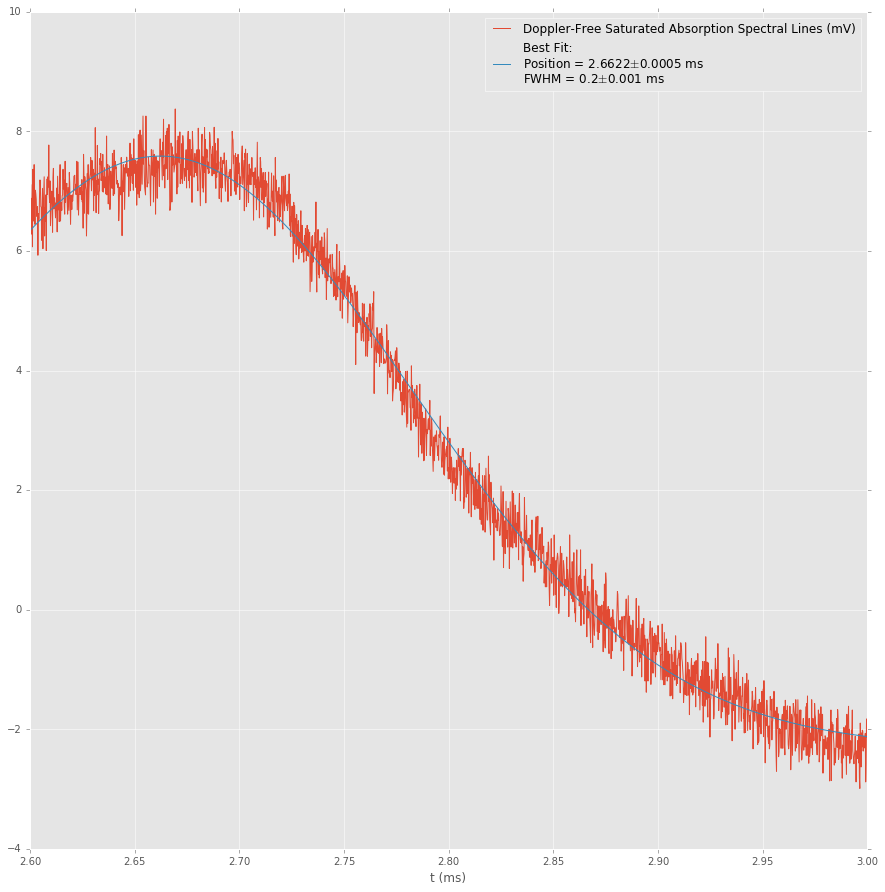
\includegraphics[width=8cm]{../Screenshots/85Rb_peak4.png}
		}%
		%
	\end{center}
	\caption{%
		Observed hyperfine peaks in ${}^{85}\text{Rb D}_2$
	}%
	\label{fig:85Hyperfine}
\end{figure}

\begin{figure}[ht!]
	\begin{center}
		%
		\subfloat[Peak 1]{%
			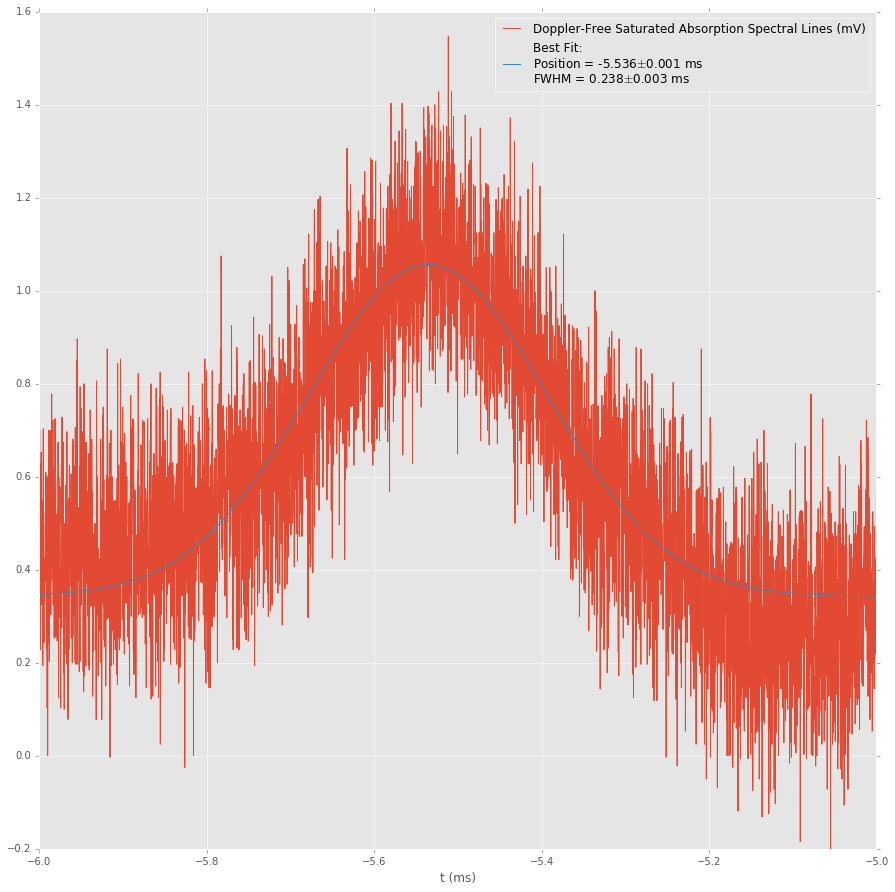
\includegraphics[width=6cm]{../Screenshots/87Rb_peak1.png}
		}%
		\subfloat[Peak 2]{%
			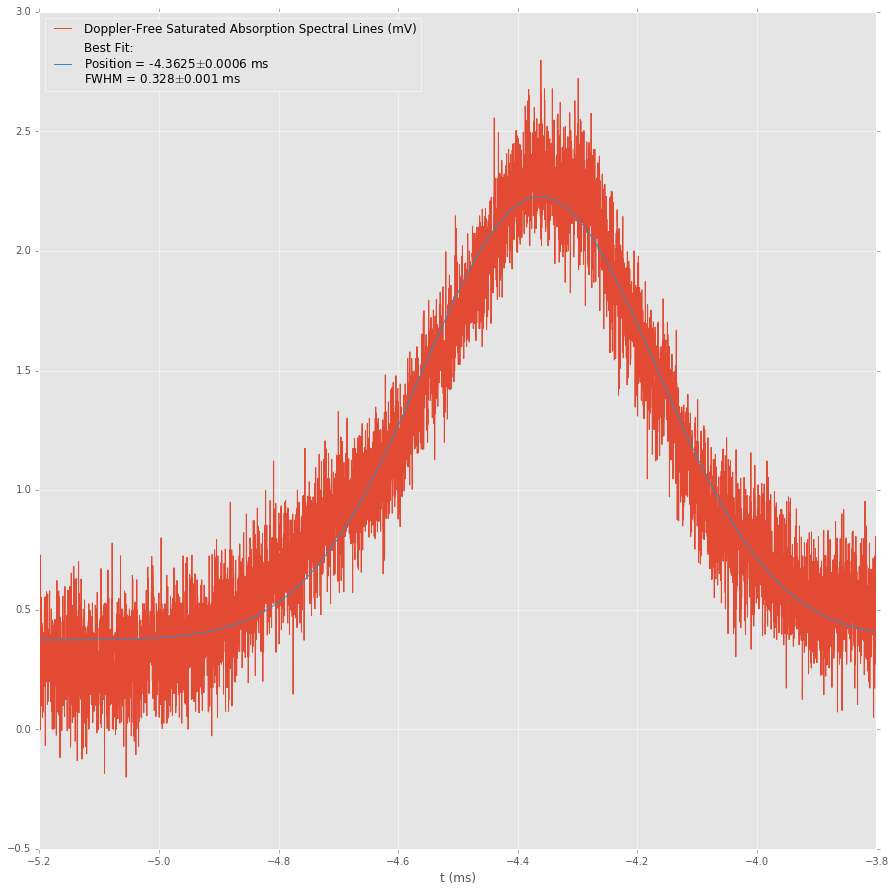
\includegraphics[width=6cm]{../Screenshots/87Rb_peak2.png}
		}\\ %  ------- End of the first row ----------------------%
		\subfloat[Peak 3]{%
			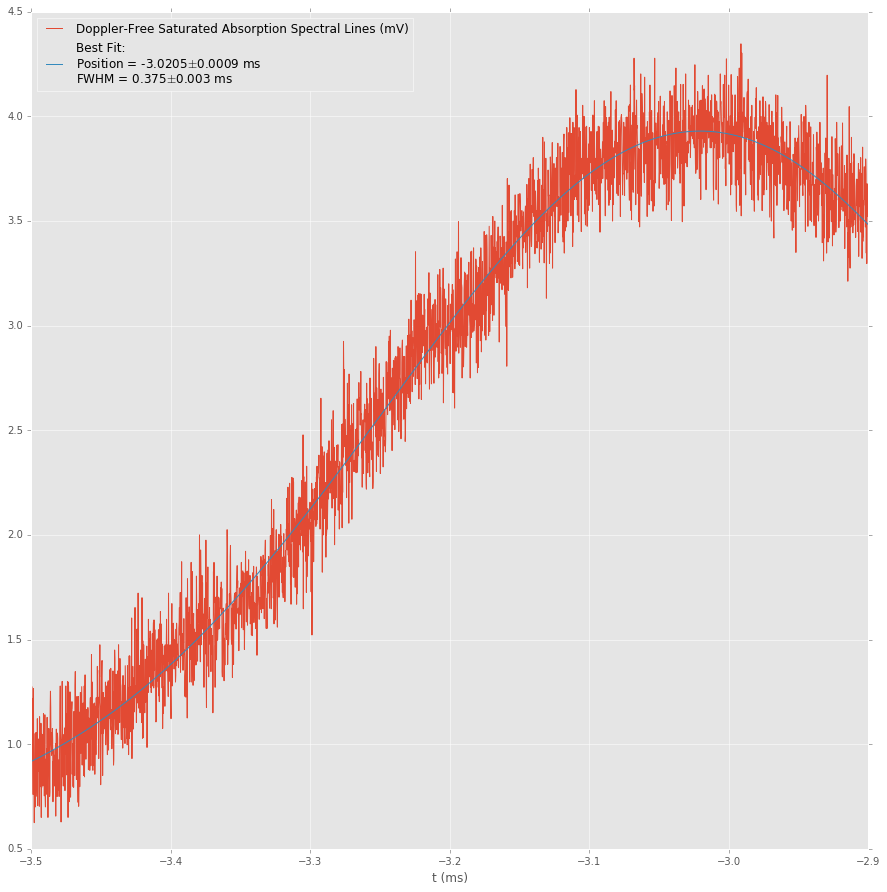
\includegraphics[width=6cm]{../Screenshots/87Rb_peak3.png}
		}%
		\subfloat[Peak 4]{%
			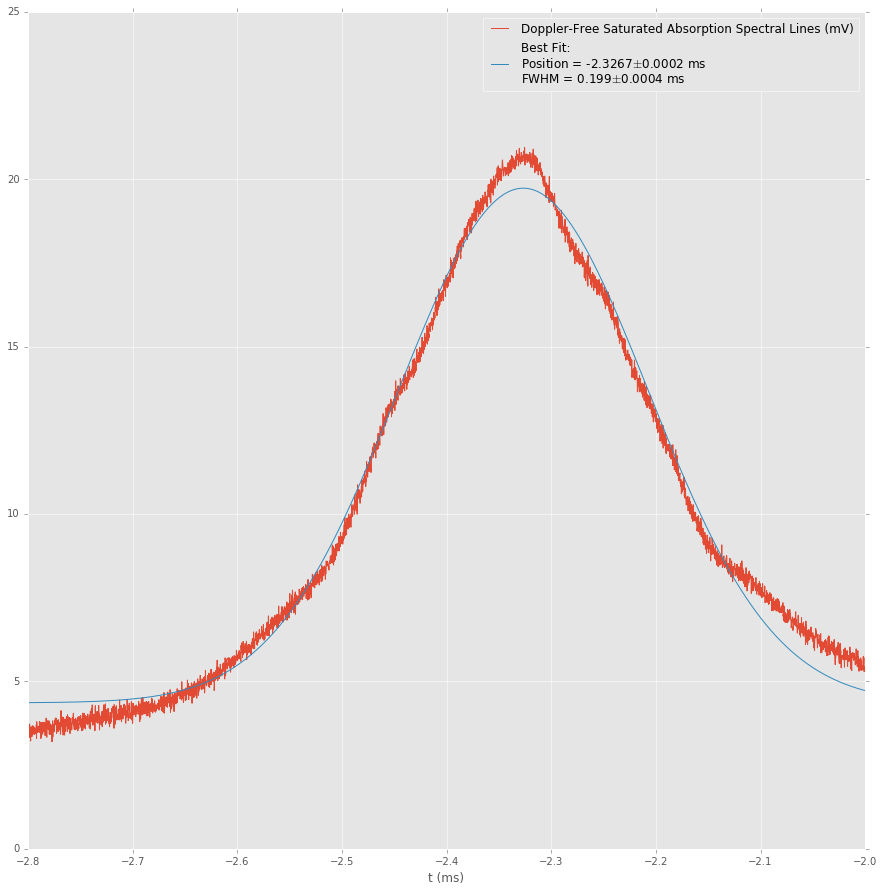
\includegraphics[width=6cm]{../Screenshots/87Rb_peak4.png}
		}\\%
		\subfloat[Peak 5]{%
			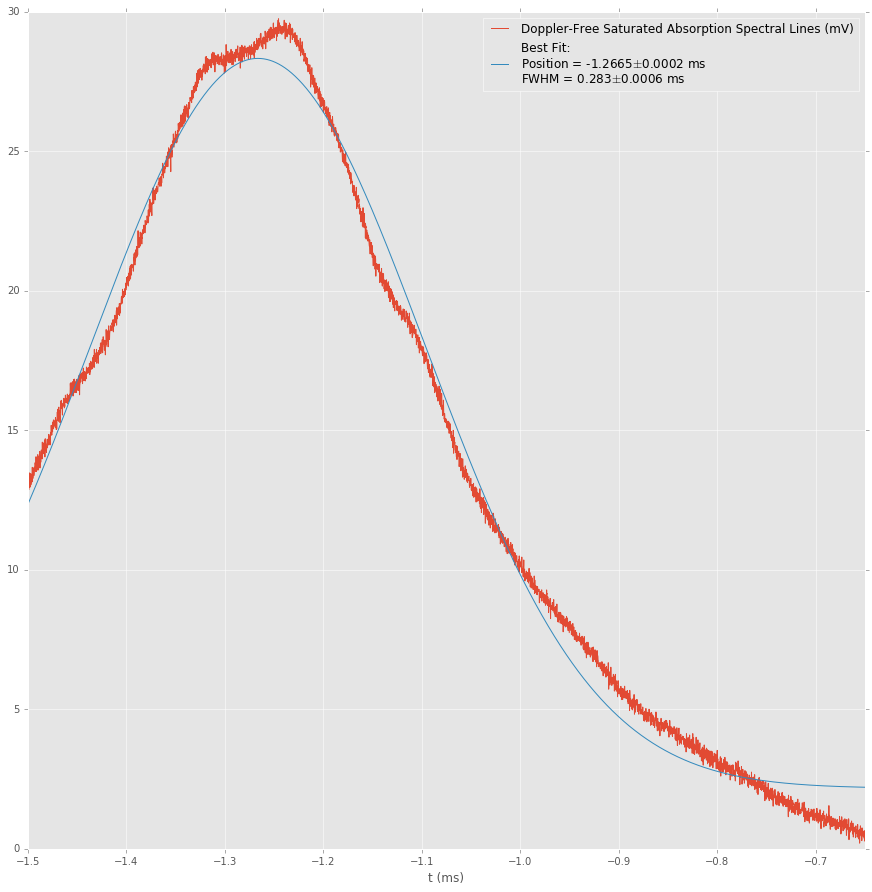
\includegraphics[width=6cm]{../Screenshots/87Rb_peak5.png}
		}%
		\subfloat[Peak 6]{%
			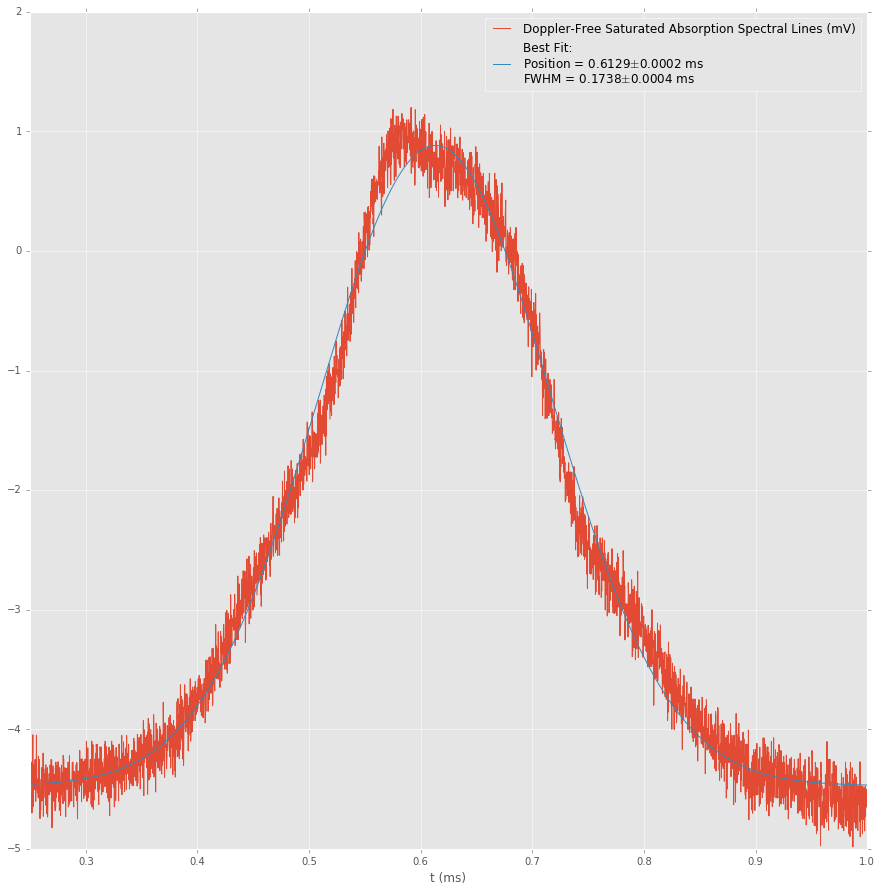
\includegraphics[width=6cm]{../Screenshots/87Rb_peak6.png}
		}%
		%
	\end{center}
	\caption{%
		Observed hyperfine peaks in ${}^{87}\text{Rb D}_2$
	}%
	\label{fig:87Hyperfine}
\end{figure}

Finally, we used numerical solvers in Python to find solutions for all combinations of the splitting equations \ref{eq:87splittings}.  We do not have sufficient data to test the splittings for $^{85}$Rb, but by we place the measured splitting lines alongside our guesses, based on the amplitude of the peaks to determine which peaks are crossovers.  Since each equation in \ref{eq:85splittings} and \ref{eq:87splittings} is an unknown in two variables, we use every combination of 2 equations with their associated transitions to solve for A and B.  We then average over all the values to obtain the reported values.  We tested our program on data from Steck\cite{steck85Rb}\cite{steck87Rb}, and obtained results that agreed with agreed upon values.  We then used this program to obtain estimates for the values A and B.  Our results are displayed below.

\begin{center}
	\begin{tabular}{| L|c | L|c |L|c|}
		\hline
		\textbf{Parameter} & {}^{85}\textbf{ Rb Expected (MHz)} & {}^{85}\textbf{ Rb Measured (MHz)}\\ 
		\hline
		\text{A} & 25.0 &  24\pm3\\ 
		\hline
		\text{B} & 25.8 & 50\pm10\\ 
		\hline
	\end{tabular}
\end{center}

\begin{center}
	\begin{tabular}{| L|c | L|c |L|c|}
		\hline
		\textbf{Parameter} & {}^{87}\textbf{ Rb Expected (MHz)} & {}^{87}\textbf{ Rb Measured (MHz)}\\ 
		\hline
		\text{A} & 84.7 &  86\pm5\\ 
		\hline
		\text{B} & 12.5 & 5\pm7\\ 
		\hline
	\end{tabular}
\end{center}


\section*{Conclusions}

 Throughout this experiment we learned about the technique of Doppler-Free Saturated Absorption Spectroscopy and used it to delve into the atomic hyperfine structure of $^{85}$Rb and $^{87}$Rb. Through meticulous alignment of the mirrors we maximized the amount of overlap between the pump beam and the probe beams allowing for hyperfine structure to be resolved. The process allows for a fine tuning to the specific frequencies associated with certain transitions of states.

Our results generally agree with what we expected from theory and values obtained from other experiments.  However, in several instances, our results did not have errors that overlapped with theoretical or established results.  While we properly propagated our error in calculations, we believe we did not properly measure or account for all error sources.  With additional time, we could track all sources of error and properly account for them, as well as ensure the results we obtained minimized this error.

Future experiments would be well advised to increase the length difference between the arms of the interferometer. Doing so will increase the number of fringes per unit time, and allow for greater precision in obtaining frequency measurements.

\bibliographystyle{unsrt}
\bibliography{DFS_ref}

\end{document}
